\providecommand{\main}{..}
\documentclass[\main/main.tex]{subfiles}

\begin{document}
\section{这里是一级标题}

\begin{figure}[htb!]
  \centering
  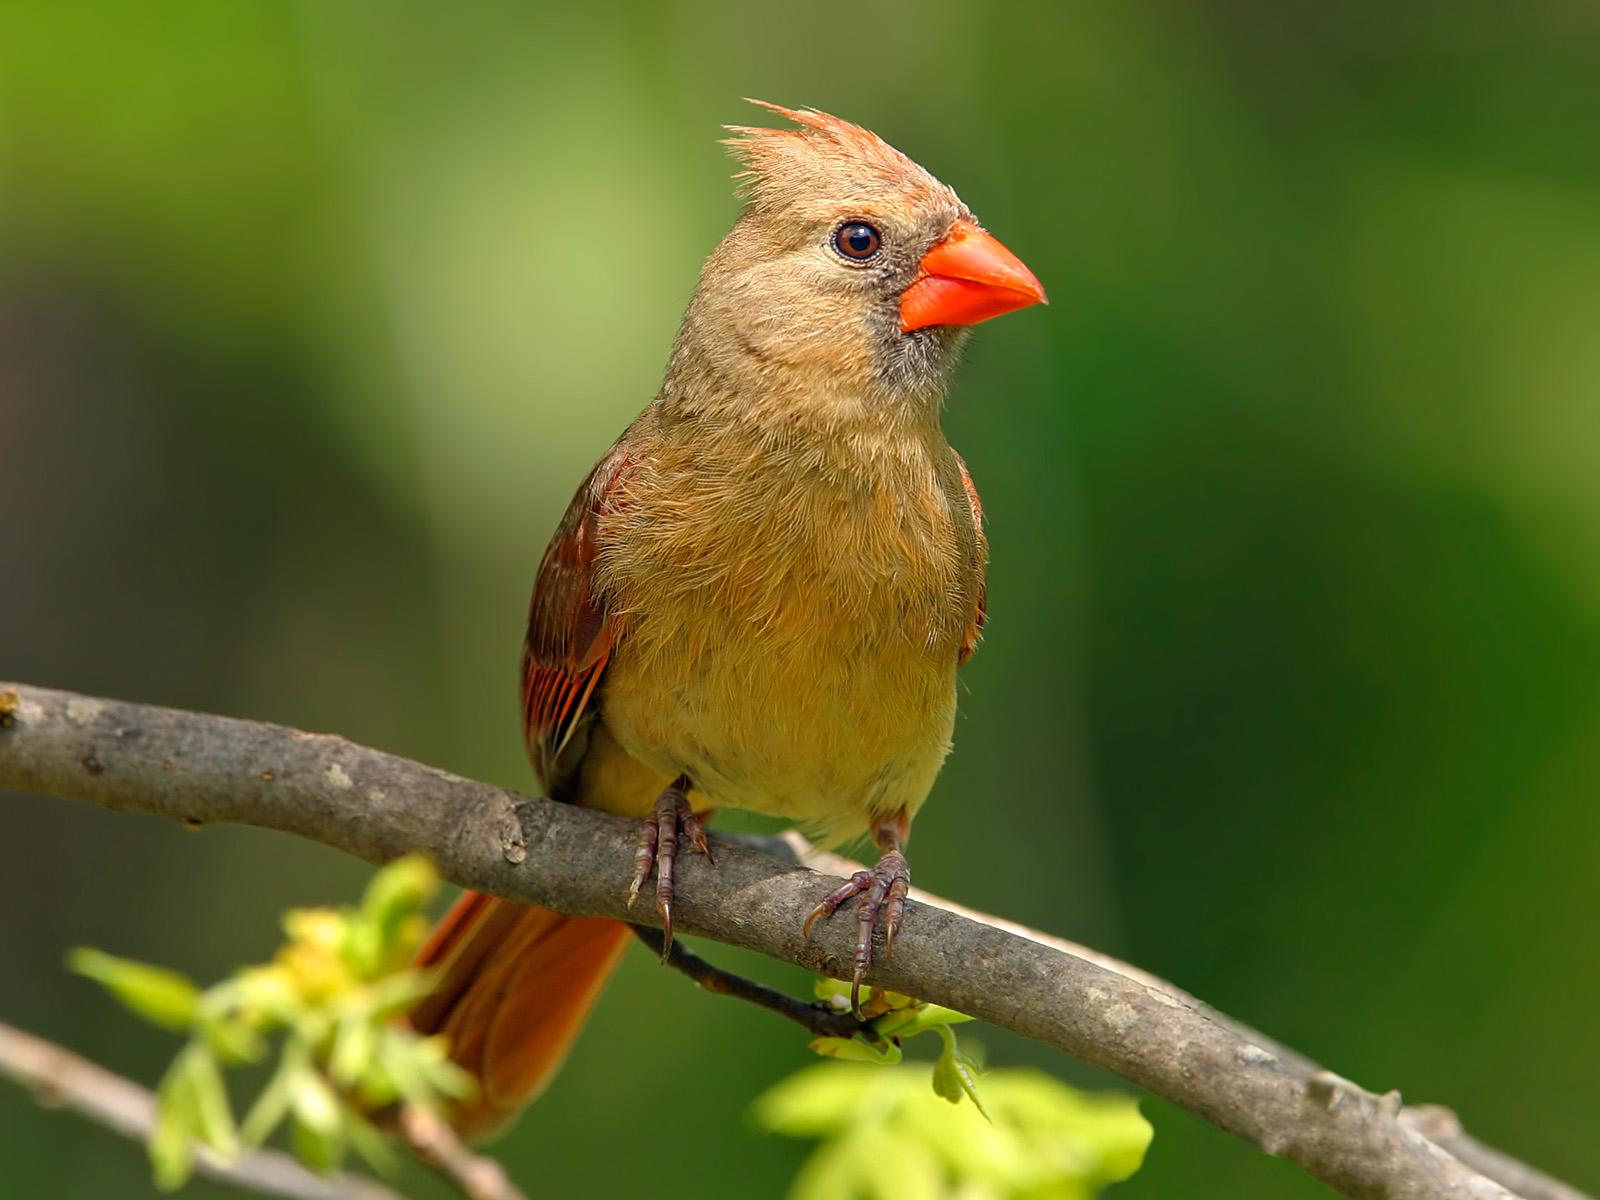
\includegraphics[width = 0.4\linewidth]{figures/test.jpg}
  \caption{这里是一张测试图片}
  \label{这里是一张测试图片}
\end{figure}

\begin{figure}[htb!]
  \centering
  \subfloat[子图1]{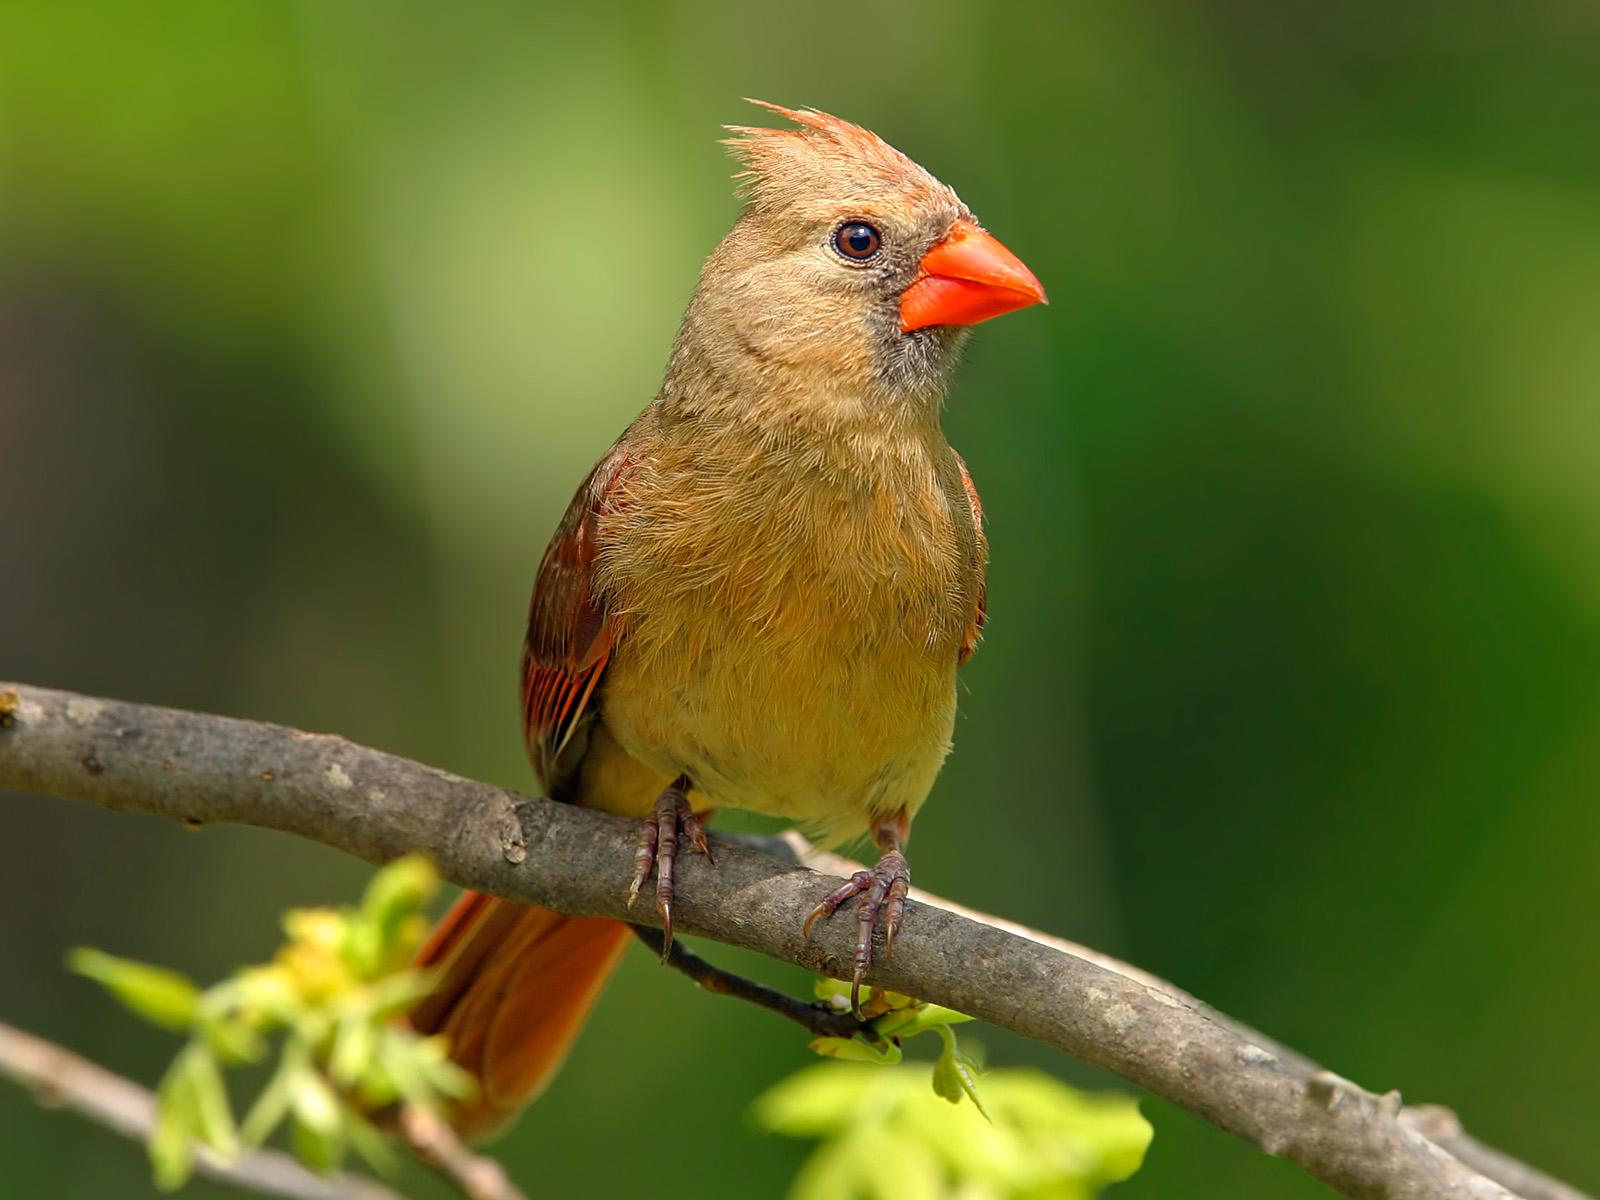
\includegraphics[width = 0.45\linewidth]{figures/test.jpg} \label{子图1}}\hspace{0.05\linewidth}
  \subfloat[子图2]{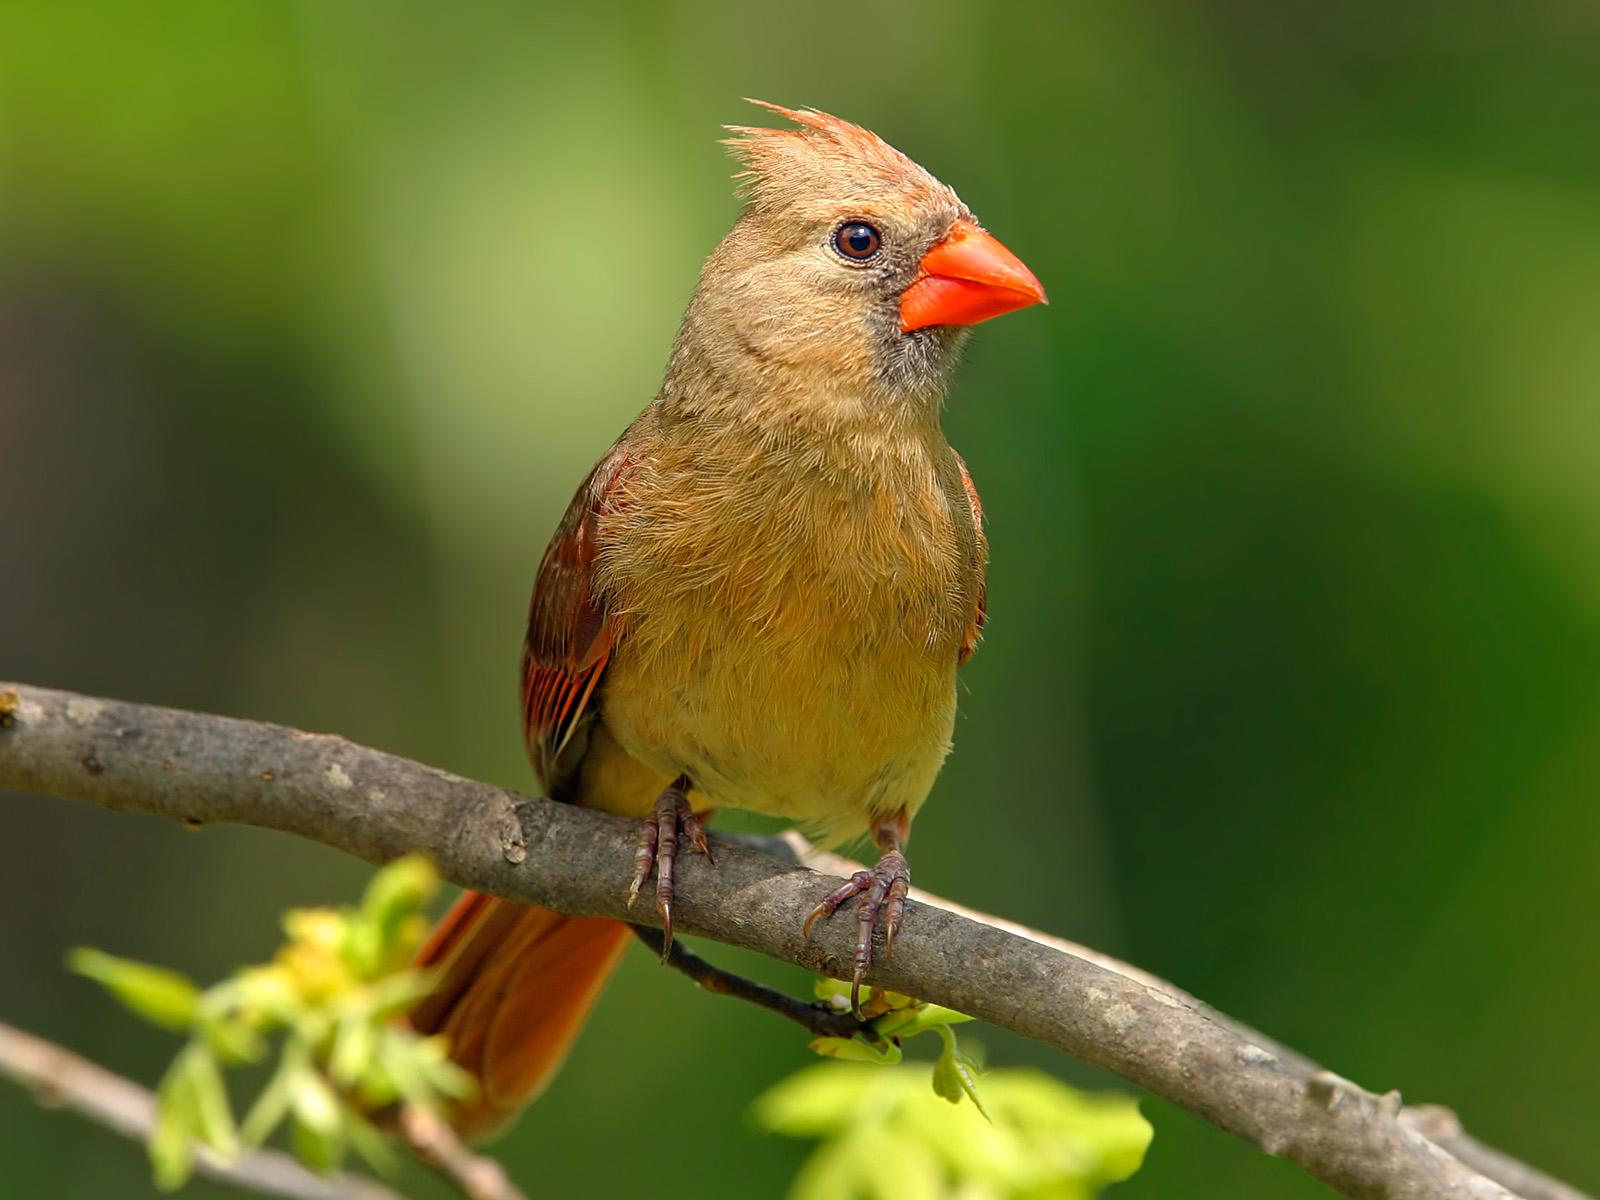
\includegraphics[width = 0.45\linewidth]{figures/test.jpg} \label{子图2}}
  \caption{这里是一个测试图}
  \label{这里是一个测试图}
\end{figure}

\cref{这里是一张测试图片} 用于测试图片的引用,而\cref{这里是一个测试图} 以及 \cref{子图1} 和 \cref{子图2} 用于测试子图的引用。

\subsection{这里是二级标题}
\subsubsection{这里是三级标题}

\begin{table}[htb!]
  \centering
  \begin{tabular}{ccc}
    \toprule
    列1 & 列2 & 列3 \\
    \midrule
    数据1 & 数据2 & 数据3 \\
    \bottomrule
  \end{tabular}
  \caption{这里是一个测试表格}
  \label{这里是一个测试表格}
\end{table}
\cref{这里是一个测试表格} 用于测试表格的引用。

\zhlipsum[3]
\begin{equation}\label{eq:example}
  f(t)={\mathcal {L}}^{-1}\{F\}(t)={\frac {1}{2\pi i}}\lim _{T\to \infty }\int _{\gamma -iT}^{\gamma +iT}e^{st}F(s)\,\mathrm {d} s,
\end{equation}
\Cref{eq:example} 用于测试公式的引用。

\end{document}